\section{CANVAS: Modelo de Negócio e Estratégia}

O Business Model Canvas~\cite{osterwalder2010} é uma ferramenta visual estratégica\footnote{O Canvas foi desenvolvido por Alexander Osterwalder e é amplamente utilizado em startups e empresas estabelecidas para modelagem de negócios.} que permite descrever, analisar e projetar modelos de negócio de forma clara e objetiva. O canvas é dividido em nove blocos fundamentais que cobrem as principais áreas de um negócio.

\begin{figure}[H]
\centering
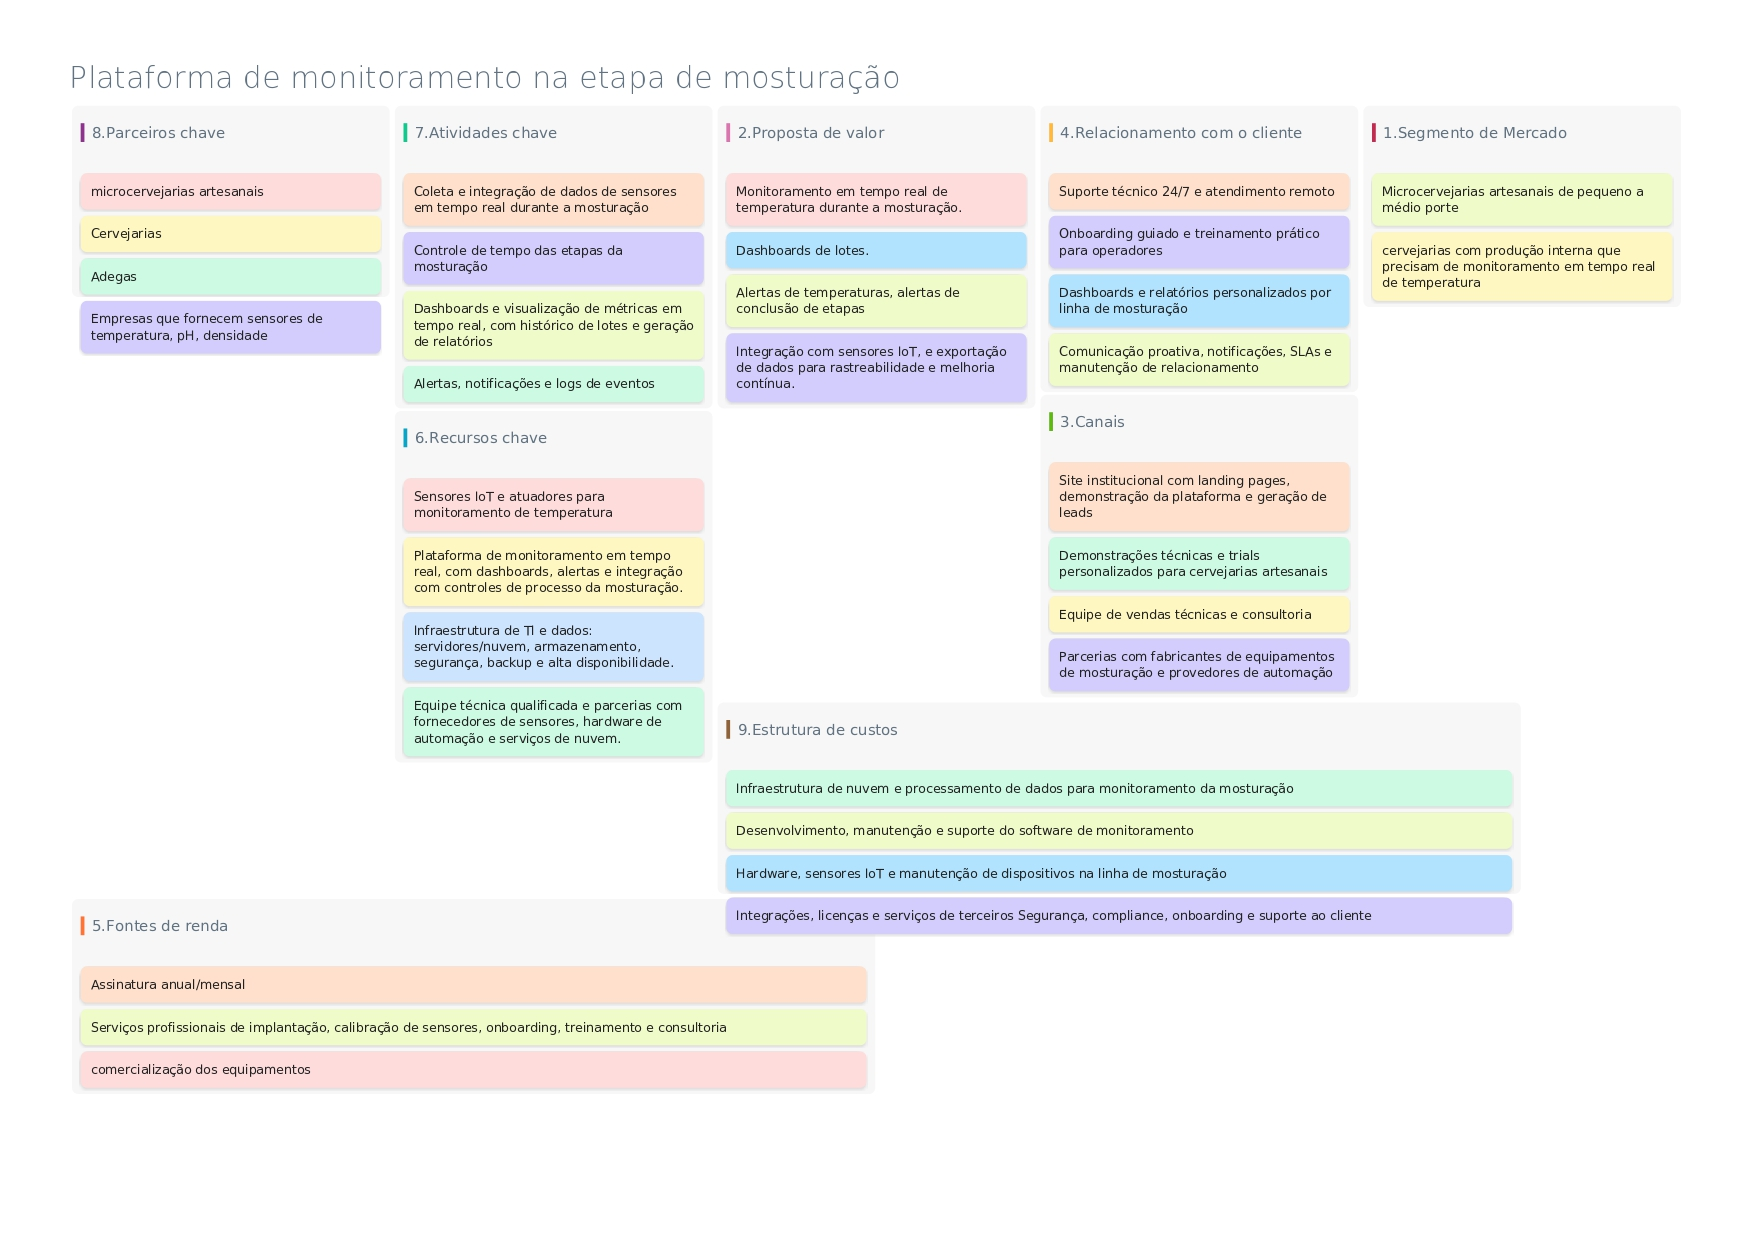
\includegraphics[width=1.1\linewidth]{imgs/canvas.jpg}
\caption{Canvas}
\label{fig:canvas}
\end{figure}

\section{SWOT}

A Análise SWOT\footnote{Também conhecida no Brasil pela sigla FOFA (Forças, Oportunidades, Fraquezas e Ameaças), a ferramenta foi desenvolvida no âmbito da administração estratégica para apoiar o planejamento corporativo e a tomada de decisão.} é uma metodologia de diagnóstico estratégico utilizada para avaliar os ambientes interno e externo de uma organização, projeto ou produto. A ferramenta estrutura-se em uma matriz quadripartida que correlaciona os pontos fortes e fracos inerentes à estrutura interna aos fatores de oportunidades e ameaças provenientes do ecossistema externo~\cite{helms2010}.

A Tabela~\ref{tab:swot} apresenta a análise do Mash na reta final do semestre. Os dados de mercado e técnicos vêm acompanhados da referência que os sustenta.

\newcommand{\swotitem}[1]{\item #1}
\newcommand{\swotcab}[2]{\cellcolor[HTML]{#1}\textbf{#2}}

\begin{table}[H]
\centering
\caption{Análise SWOT do Projeto}
\label{tab:swot}
\renewcommand{\arraystretch}{1.2}
\begin{tabular}{|p{0.46\textwidth}|p{0.46\textwidth}|}
\hline
\multicolumn{2}{|c|}{\textbf{FATORES INTERNOS}} \\
\hline
\swotcab{E3F4EA}{FORÇAS (Strengths)} & \swotcab{FDF3D8}{FRAQUEZAS (Weaknesses)} \\
\hline
\begin{itemize}[leftmargin=*, nosep, after=\vspace{-\baselineskip}]
\swotitem{API com autenticação JWT, senhas guardadas com hash Argon2 e isolamento entre usuários}
\swotitem{Receitas, rampas de temperatura e lotes ligados da tela ao banco de dados}
\swotitem{Schema do banco criado por \textit{migrations} versionadas}
\swotitem{API e frontend publicados em ambiente de nuvem}
\swotitem{Decisões e recorte do semestre registrados em um só lugar}
\end{itemize}
&
\begin{itemize}[leftmargin=*, nosep, after=\vspace{-\baselineskip}]
\swotitem{Sem testes automatizados; a validação é manual, por exceção registrada}
\swotitem{Classificação automática do teste do iodo não implementada; neste semestre o teste é uma simulação na interface}
\swotitem{Equipe de quatro integrantes, com dois dedicados à programação}
\end{itemize}
\\
\hline
\multicolumn{2}{|c|}{\textbf{FATORES EXTERNOS}} \\
\hline
\swotcab{E5F0F8}{OPORTUNIDADES (Opportunities)} & \swotcab{FDECEA}{AMEAÇAS (Threats)} \\
\hline
\begin{itemize}[leftmargin=*, nosep, after=\vspace{-\baselineskip}]
\swotitem{1.949 cervejarias registradas no Brasil, com crescimento de 5,5\% em 2024 \cite{MAPA2025}}
\swotitem{EXPOBEER Vale do Ribeira e a produção regional de cerveja artesanal \cite{ExpoBeerEvento2025}}
\swotitem{A banca avalia o fluxo principal demonstrado, e não funcionalidades fora do recorte}
\end{itemize}
&
\begin{itemize}[leftmargin=*, nosep, after=\vspace{-\baselineskip}]
\swotitem{Prazo do depósito do projeto em 03/11/2026}
\swotitem{O plano gratuito do Render desliga a API após 15 minutos sem uso, e ela leva cerca de 1 minuto para voltar}
\swotitem{A iluminação do ambiente altera a leitura da cor do iodo \cite{li2025starch}}
\end{itemize}
\\
\hline
\end{tabular}
\end{table}

\subsection{Recomendações Estratégicas}

Com base na análise SWOT, a equipe definiu as estratégias da reta final:

\begin{itemize}
\item \textbf{Forças + Oportunidades:} demonstrar o ciclo completo, do login ao lote, com usuário, receita e lote já cadastrados.
\item \textbf{Fraquezas + Oportunidades:} congelar o escopo e executar na véspera um roteiro de validação manual do fluxo principal.
\item \textbf{Forças + Ameaças:} manter um ambiente local com as \textit{migrations} aplicadas e os dados de demonstração, e gravar um vídeo do fluxo como plano B.
\item \textbf{Fraquezas + Ameaças:} retirar do semestre o teste do iodo automatizado e apresentar a simulação de interface já pronta.
\end{itemize}
